\chapter{Descrizione a B-splines di una curva nel piano}\lb{BSC}

%==========================================================================================
\section{Introduzione}

Descrivere la curva ${\bf r}(u,t)$ in termini di spline significa determinare le due funzioni
$x(u,t)$ e $y(u,t)$, componenti di ${\bf r}$, note appunto come splines, ottenute dalla
composizione di segmenti di funzioni polinomiali o {\it spans}.
Le {\it B-splines} rappresentano una particolare classe di splines in cui la funzione 
$x(u,t)$ \e ottenuta come combinazione lineare di $N_B$ funzioni base (da cui B-spline)
$B_i(u)$, e con combinatori i {\it control points} $x_i(t)$, $i=0,\dots,N_B-1$
\be
x(u,t)\,=\,\sum_{i=0}^{N_B-1}\,B_i(u)\,x_i(t).
\ee
   
Ciascuna base $B_i$ \e definita dall'unione di $d$ segmenti di polinomio di ordine $d$ 
o di grado $d-1$ a supporto finito dato dall'intervallo $[u_i,u_{i+d}[$
dove ciascun $u_i$ rappresenta il {\it nodo} o {\it knot} $i-esimo$ della splines.  
Nel caso particolare delle {\it B-splines uniformi} la sequenza di nodi $\{u_i\}$ \e
equispaziata per cui si considera ${\bf r}(s,t)$ per ciascun span, con 
$$
s=\frac{u-u_i}{u_{i+1}-u_i}\in [0,1[ \quad e \quad u\,\in\,[\,u_i,u_{i+1}\,[.
$$

Si fissa inoltre che ciascuna base presenti anche delle condizioni di regolarit\a, in
particolare che siano continue le prime $d-2$ derivate su tutto il supporto;
in questo modo anche la curva ${\bf r}(u,t)$ \e una funzione $C^{d-2}$ su tutto il dominio.

%----------------------------------------------------------------------------------------
\section{B-splines lineari}

\begin{figure}[tbp]
 \centerline{
  \psfig{file="./images/linearBs.ps",height=6cm,clip=}}
 \caption[B-spline lineari]
  {Esempio di interpolazione con B-splines lineari in cui sono tratteggiate due basi.}
 \lb{Bslin}
\end{figure}

Per comprendere il significato e le propriet\a dei control points e delle basi \e conveniente
considerare dapprima il caso di $d=2$, il pi\u semplice rispetto alle condizioni di
regolarit\a fissate, che corrisponde alle {\it B-splines lineari} (Figura \r{Bslin}).
Il risultato \e l'interpolazione lineare degli stessi punti di controllo $x_i$ dove le basi
$B_i$ sono definite su un intervallo di ampiezza pari a $2$ e hanno forma triangolare.
Fissati quindi $m$ punti o vertici di controllo si hanno $m-1$ segmenti di retta le cui 
equazioni sono esprimibili rispetto al parametro $s$
\beqa
x_{i-1}(s) & = & \,(1-s)\,x_{i-2}\,+\,s\,x_{i-1} \lb{segint}\\
x_i(s) & = & \,(1-s)\,x_{i-1}\,+\,s\,x_i \nonumber\\
x_{i+1}(s) & = & \,(1-s)\,x_{i}\,+\,s\,x_{i+1} \nonumber\\ 
x_{i+2}(s) & = & \,(1-s)\,x_{i+1}\,+\,s\,x_{i+2} \nonumber
\eeqa
$$
con \quad s=\frac{u-u_i}{u_{i+1}-u_i} \quad e \quad u\,\in\,[\,u_i,u_{i+1}\,[
$$
per cui ai due estremi per $s=0$ e $s=1$ corrispondono a $x(0)=x_{i-1}$ e $x(1)=x_i$
rispettivamente\footnotemark.

\footnotetext{Si \e valutato $x(1)$ anche se si \e definito $s$ nell'intervallo aperto
superiormente $[\,0,1\,[$; sarebbe possibile considerare l'intervallo chiuso in quanto
le funzioni splines qui definite sono almeno continue. Cos\iac\,facendo invece si mantengono
gli spans distinti senza punti in comune.}

In Figura \r{Bslin} sono stati tracciati i contributi di $x_{i-1}$ e $x_i$ ricavati
dalle equazioni (\r{segint}) dove si vede che ciascun control points interviene nella
definizione dei due spans adiacenti che lo condividono.
Le due funzioni tratteggiate hanno la stessa forma e altezza che varia con la posizione
dei control points che \e possibile pensarle come le basi $B_i$ di altezza unitaria
scalate dai punti di controllo $x_i$.
Ne risulta che modificando la posizione di un solo vertice si hanno delle variazioni
locali della curva complessiva, per cui si parla di {\it controllabilit\a locale}, che
rappresenta una delle propriet\a fondamentali delle splines.

E' possibile allora esprimere l'equazione del segmento o span (\r{segint}) che collega i due
vertici $x_{i-1}$ e $x_i$ come la combinazione lineare di due basi $B_{i-1}$ e $B_i$
\be
x_i(u)\,=\,x_{i-1}\,B_{i-1}(u)+\,x_i\,B_i(u)
\lb{comb}
\ee
l'imitatamente all'intervallo $u_i \leq u \leq u_{i+1}$ in cui \e definito lo span, con
\[
B_i(u)\,=\,\cases{
           {\ds\frac{u-u_i}{u_{i+1}-u_i}} & $u_i \leq u \leq u_{i+1}$ \cr
              &   \cr                                                    
           {\ds\frac{u_{i+2}-u}{u_{i+2}-u_{i+1}}} & $u_{i+1} \leq u \leq u_{i+2}$. \cr}
\]

\vs(5)

Quanto appena visto pu\o essere esteso all'intera funzione $x(u)$ (o $x(s)$ nel caso di
B-splines uniformi) e quindi anche a $y(s)$; per cui l'intera curva ${\bf r}(u,t)$ risulta
\be
{\bf r}(u,t)\,=\,\sum_{i=0}^{N_B-1}\,{\bf x}_i(t)\,B_i(u) \qquad {\bf x}_i=(x_i,y_i)
\lb{curva}
\ee
oppure
\be
{\bf r}(s,t)\,=\,\sum_{i=0}^{N_B-1}\,{\bf x}_i(t)\,B(s-i)
\ee
nel caso di B-splines uniformi dove la base $B_i$ \e ottenuta semplicemente traslando
la base di riferimento $B$.

%=========================================================================================
\section{B-splines cubiche uniformi}

Consideriamo ora il caso delle {\it B-spline cubiche} ovvero splines ottenute dalla combinazione
di funzioni base che sono costituite da tratti di polinomi cubici ($d=4$).
Inoltre si assuma definitivamente l'ipotesi di splines uniformi per cui i nodi o knots
$u_i$ sono equispaziati; in particolare \e possibile considerarli posti a distanza unitaria
e quindi possono essere sostituiti con una sequenza di interi come in Figura (\r{Bscubic}).
Ciascuna base perci\o \e ottenuta come traslazione di una base di riferimento, come
accennato precedentemente.

\begin{figure}[tbp]
 \centerline{
  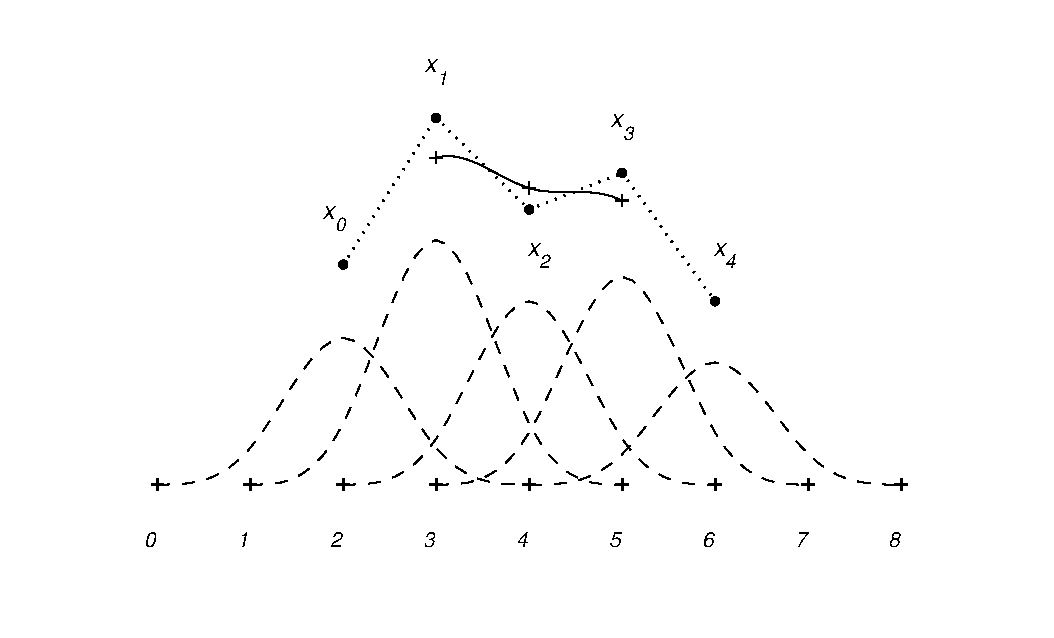
\psfig{file="./images/cubicBs.eps",height=6cm,clip=}}
 \caption[Curva a B-splines cubiche uniformi]
  {Tratto di curva ottenuto dalla combinazione delle funzioni base date dalle B-splines
   cubiche secondo i control points $x_i$. Nel caso di splines uniformi ciacuna base
   $B_i$ \e ottenuta come traslazione di una base di riferimento $B$.}
 \lb{Bscubic}
\end{figure}

A differenza del caso delle B-spline lineari, quelle cubiche non passano
necessariamente per i control points ma al pi\u possono avvicinarsi; tutto dipende dal
numero dei punti di controllo e dalla loro disposizione (nel caso in cui questi siano
allineati la spline deve necessariamente attraversarli).

\begin{figure}[tbp]
 \centerline{
  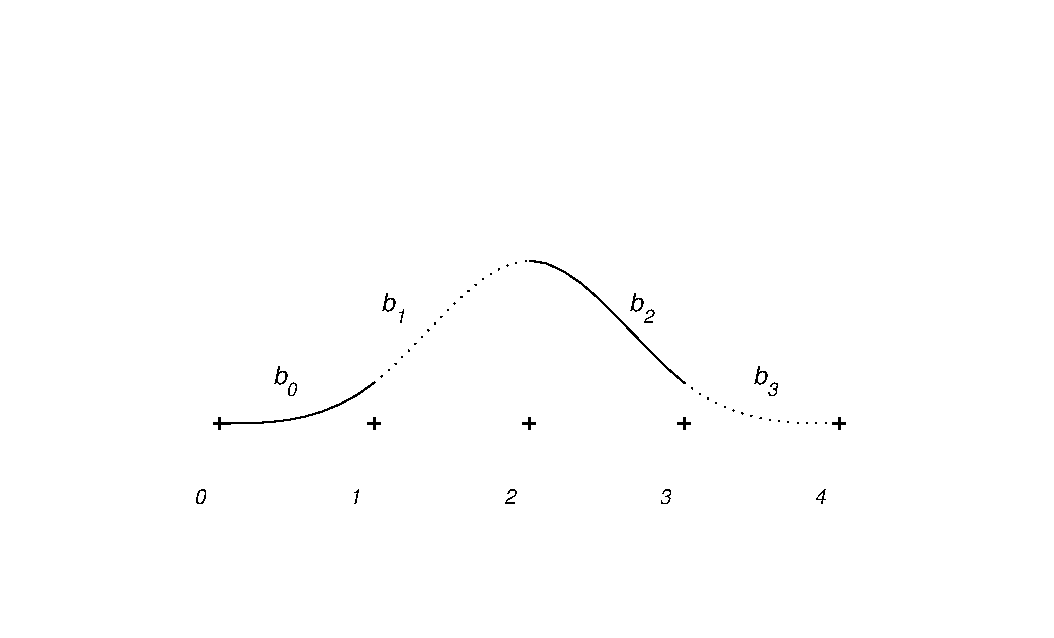
\psfig{file="./images/Bcubic.eps",height=6cm,clip=}}
 \caption[B-spline cubica di riferimento]
  {Base di una B-spline cubica uniforme: \e una curva a tratti di polinomi cubici a supporto
   finito pari a $d=4$ volte la distanza fra due nodi.}
 \lb{BaseBc}
\end{figure}

Dalla Figura \r{Bscubic} si possono individuare alcune caratteristiche della curva ottenuta
dalla combinazione delle B-splines cubiche in particolare, ma che \e possibile estendere
all'intera famiglia delle B-splines:

fissati $m$ {\it control points}, con indice $i=0,\dots,m-1$ 
\ben
\im si hanno $m$ basi $B_i$;
\im la curva \e scomponibile in $m-3$ {\it spans}
\im che si appoggiano su $m-2$ nodi;
\im la spline generata si sviluppa quindi a partire dal quarto nodo $u_3$ e termina in
    corrispondenza del nodo $u_m$.
\een


In Figura \r{BaseBc} \e rappresentata la base $B(s)$ di riferimento menzionata nella
quale sono indicati con diverso tratto i quattro segmenti di polinomio cubico 
\be
a_js^3\,+\,b_js^2\,+\,c_js\,+\,d_j \qquad 0 \leq j \leq 3. 
\ee
Ne risultano quindi $16$ incognite date dai coefficienti dei polinomi che possono essere
individuati in modo univoco considerando i vincoli che derivano dalla regolarit\a imposta
precedentemente alle curve a B-spline, ovvero che siano $C^2$ su tutto il dominio:
\bary(3)
0\,=\,b_0(0)      & 0\,=\,b_0^{(1)}(0)            & 0\,=\,b_0^{(2)}(0)            \\
b_0(1)\,=\,b_1(0) & b_0^{(1)}(1)\,=\,b_1^{(1)}(0) & b_0^{(2)}(1)\,=\,b_1^{(2)}(0) \\
b_1(1)\,=\,b_2(0) & b_1^{(1)}(1)\,=\,b_2^{(1)}(0) & b_1^{(2)}(1)\,=\,b_2^{(2)}(0) \\
b_2(1)\,=\,b_3(0) & b_2^{(1)}(1)\,=\,b_3^{(1)}(0) & b_2^{(2)}(1)\,=\,b_3^{(2)}(0) \\
b_3(1)\,=\,0      & b_3^{(1)}(1)\,=\,0            & b_3^{(2)}(1)\,=\,0            
\eary
che come si nota impongono la continuit\a fino alla derivata seconda ($d-2$) compresa nei
punti di raccordo o {\it breakpoints} tra le curve polinomiali valutati per $s=0$ e $s=1$.

Un'ultima condizione \e fissata imponendo che
$$
b_0(0)\,+\,b_1(0)\,+\,b_2(0)\,+\,b_3(0)\,=\,1
$$
che si riduce a 
$$
b_1(0)\,+\,b_2(0)\,+\,b_3(0)\,=\,1
$$
dato che \e gi\a stato fissato $b_0(0)=0$.

Risolvendo le equazioni nei coefficienti incogniti $a_j$, $b_j$, $c_j$, $d_j$ per i quattro
segmenti che compongono $B$ si ricava
\beqa
b_0(s) & = & \frac{1}{6}\,s^3 \nonumber\\
 & \nonumber\\
b_1(s) & = & \frac{1}{6}\,\Big(\,-3s^3+3s^2+3s+1\,\Big) \nonumber\\
 & \lb{polcubic}\\
b_2(s) & = & \frac{1}{6}\,\Big(\,3s^3-6s^2+4\,\Big) \nonumber\\
 & \nonumber\\
b_3(s) & = & \frac{1}{6}\,\Big(\,-s^3+3s^2-3s+1\,\Big) \nonumber
\eeqa

Da queste \e possibile ottenere un'interessante espressione per lo {\it span} $i-esimo$ definito
sull'intervallo $[u_i,u_{i+1}[$.
A partire dalla (\r{curva}), trascurando per semplicit\a la variabile temporale,
\be
{\bf r}(u)\,=\,\sum_{i=0}^{N_B-1}\,{\bf x}_i\,B_i(u);
\ee
e tenendo presente che la base $B_i$ e non nulla solo su $[u_i,u_{i+d}[$, allora nell'inter-vallo
$[u_i,u_{i+1}[$ intervengono solo un numero finito, pari a $d$, di basi 
\beqa
{\bf r}_i(u) & = & \sum_{j=0}^{3}\,{\bf x}_{i-j}\,B_{i-j}(u)\,= \nonumber\\
             &   & \\
             & = & {\bf x}_{i}\,B_{i}(u)\,+\,{\bf x}_{i-1}\,B_{i-1}(u)\,+\,
                   {\bf x}_{i-2}\,B_{i-2}(u)\,+\,{\bf x}_{i-3}\,B_{i-3}(u) \nonumber
\eeqa

Inoltre, limitatamente all'intervallo considerato, la $B_i$ contribuisce con il tratto di
polinomio $b_i$ per cui l'espressione si semplifica ulteriormente nella
\beqa
{\bf r}_i(s) & = & \sum_{j=0}^{3}\,{\bf x}_{i-j}\,b_{j}(s)\,= \nonumber\\
             &   & \lb{rsempl}\\
             & = & {\bf x}_{i}\,b_{0}(s)\,+\,{\bf x}_{i-1}\,b_{1}(s)\,+\,
                   {\bf x}_{i-2}\,b_{2}(s)\,+\,{\bf x}_{i-3}\,b_{3}(s) \nonumber
\eeqa
per ogni quaterna $[\,{\bf x}_i,{\bf x}_{i-1},{\bf x}_{i-2},{\bf x}_{i-3}\,]$ di
{\it control points}.

\boss
Il vantaggio di quest'ultima espressione \e che pu\o essere convenientemente espressa in
forma matriciale.
Riordinando i termini della (\r{rsempl}) nella forma
\be
{\bf r}_i(s)\,=\,{\bf x}_{i-3}\,b_{3}(s)\,+\,{\bf x}_{i-2}\,b_{2}(s)\,+\,
                 {\bf x}_{i-1}\,b_{1}(s)\,+\,{\bf x}_{i}\,b_{0}(s) 
\ee
la si pu\o scrivere come prodotto di vettori
\be
{\bf r}_i(s)\,=\,{\bf b}(s)\,{\bf x}_i\,=\,
                 \qmatrix{b_3(s) & b_2(s) & b_1(s) & b_0(s)\cr}\,
                 \qmatrix{{\bf x}_{i-3} \cr
                          {\bf x}_{i-2} \cr
                          {\bf x}_{i-1} \cr
                          {\bf x}_{i} \cr}.
\ee
Espandendo i termini $b_j$ il primo vettore risulta
\be
{\bf b}(s)\,=\,{\bf s}^T\,{\bf M}\,=\,\frac{1}{6}
               \qmatrix{s^3 & s^2 & s & 1 \cr}\,
               \smatrix{4}{ -1 &  3 & -3 &  1 \cr
                             3 & -6 &  3 &  0 \cr
                            -3 &  0 &  3 &  0 \cr
                             1 &  4 &  1 &  0 \cr} 
\ee   
e quindi concludendo

\be
{\bf r}_i(s)\,=\,\frac{1}{6}\,{\bf s}^T\,{\bf M}\,{\bf x}_i
\lb{cBsmat}
\ee
\eoss

\begin{figure}[tbp]
 \centerline{
  \psfig{file="./images/conv_h1.eps",height=6cm,clip=}}
 \caption[Curva 2D a B-splines ]
  {Esempio di curva bidimensionale chiusa a B-splines cubiche uniformi con poligono dei
   control points.}
 \lb{curva2d}
\end{figure}

%=======================================================================================
\section{Alcune propriet\a delle B-splines}

%---------------------------------------------------------------------------------------
\subsection{Convex hull}

\begin{figure}[tbp]
 \centerline{
  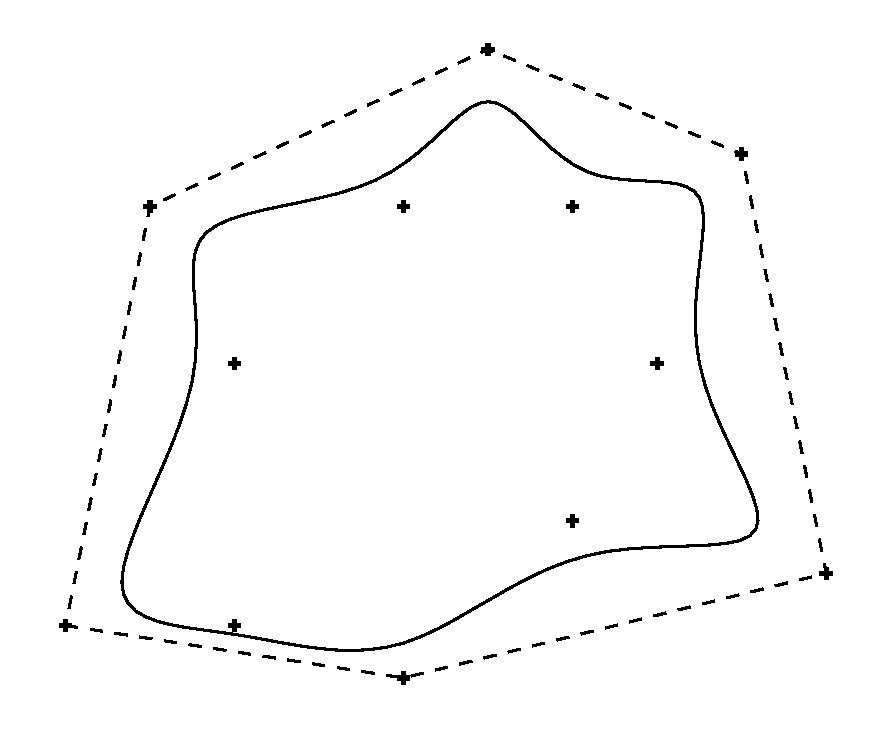
\psfig{file="./images/conv_h2.eps",height=6cm,clip=}}
 \caption[Convex Hull]
  {La regione convessa, convex hull, che contiene tutti i control points e la curva di 
   figura (\r{curva2d}).}
 \lb{convhull}
\end{figure}

In figura (\r{convhull}) \e rappresentato la {\it convex hull} dell'insieme $Q$ dei
{\it control points} definita come il pi\u piccolo poligono convesso tale per cui tutti 
i punti di $Q$ o sono interni o al pi\u appartengono al bordo.

\vs(5)

Dalla definizione di insieme convesso
\bdf
{\bf Insieme convesso.}\par
Si dice che un sottoinsieme $A$ di uno spazio vettoriale \e convesso quando verifica la
condizione:
\be
\alpha\,{\bf x}_1\,+\,(1-\alpha)\,({\bf x}_2-{\bf x}_1)\,\in\,A \qquad 
 \forall\,{\bf x}_1,{\bf x}_2\in A \quad \forall\,\alpha\in [0,1]
\ee
\edf
(Nel nostro caso lo spazio considerato \e $\M(R)^2$ e l'insieme $A$ \e la convex hull).

\e possibile ricavare la condizione che caratterizza la convex hull in funzione dei
control points, ovvero
\bpr
\par
Ciascun punto {\bf p} della convex hull pu\o essere espresso come combinazione lineare
convessa dei control points $[{\bf x}_0,\dots,{\bf x}_{m-1}]$
\be
{\bf p}\,=\,\sum_{i=0}^{m-1}\,w_i\,{\bf x}_i\, ,\qquad
w_i \geq 0\quad\forall i \quad e \quad \sum_{i=0}^{m-1}\,w_i\,=\,1
\ee
\epr   

Si consideri lo span definito dai control points $[{\bf x}_0,{\bf x}_1,{\bf x}_2,{\bf x}_3]$
di Figura \r{Bscubic}; questi risulta contenuto nella convex hull definita dai suoi
$4$ control points nell'ordine, antiorario, $\{{\bf x}_0,{\bf x}_2,{\bf x}_3,{\bf x}_1\}$.
Infatti vale la proposizione precedente in quanto si verifica dalle (\r{polcubic}) che
\be
\sum_{j=0}^{3}\,b_j(s)\,=1 \qquad \forall\quad s \in \,[0,1[
\lb{sumunit}
\ee
ed inoltre $b_j(s)$ \e non negativa, quindi i nostri $w_i$ sono proprio i $b_j$.

In base a questi risultati, noto il poligono dei control points, \e possibile conoscere
lo spazio in cui si trova la curva a B-splines.
In particolare la B-spline approssima in modo regolare le variazioni del poligono
dei control points.

%---------------------------------------------------------------------------------------
\subsection{Invarianza alle traslazioni}

Con tale propriet\a si vuole indicare che anche se i {\it control points} ${\bf x}_i$ vengono
traslati della stessa quntit\a ${\bf v}$ la nuova curva descritta ${\bf r_v}$ \e ottenuta
applicando la stessa traslazione a tutti i punti della curva originaria ${\bf r}$.

\be
{\bf r_v}(u)\,=\,\sum_{i=0}^{m-1}\,B_i(u)\,({\bf x}_i+{\bf v})\,=\,
                 \sum_{i=0}^{m-1}\,B_i(u)\,{\bf x}_i\,+\,
                 {\bf v}\,\sum_{i=0}^{m-1}\,B_i(u)            
\ee

Per la propriet\a precedente (\r{sumunit}) la seconda sommatoria \e pari a $1$ per cui risulta
\be
{\bf r_v}(u)\,=\,\sum_{i=0}^{m-1}\,B_i(u)\,{\bf x}_i\,+\,{\bf v}\,=\,
                 {\bf r}(u)\,+\,{\bf v} \qquad \forall\, u
\ee

%---------------------------------------------------------------------------------------
\subsection{Invarianza alle rotazioni e alle omotetie}

\begin{figure}[tbp]
 \centerline{
  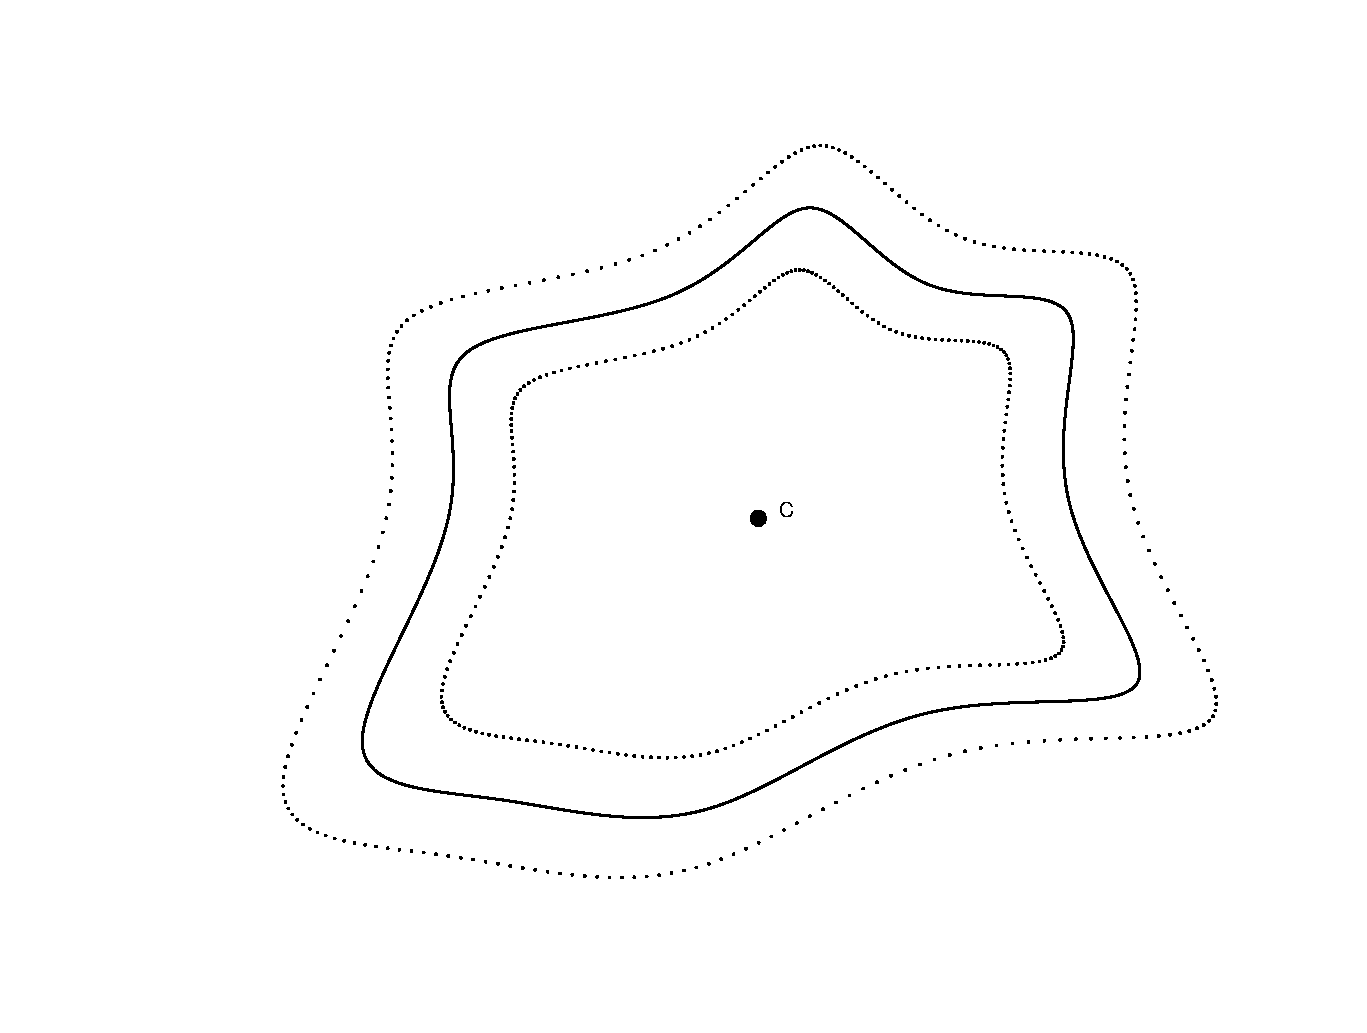
\psfig{file="./images/omotetia.eps",height=6cm,clip=}}
 \caption[Omotetia rispetto al centroide dei control points]
  {Due casi di omotetia rispetto al centroide ${\bf c}$ dei {\it control points}: una
   {\it dilatazione} e una {\it contrazione}}
 \lb{omotetia}
\end{figure}

E' possibile verificare la stessa invarianza sia per le rotazioni sia per le omotetie 
(dilatazioni o contrazioni).

\bi
\im {\it Rotazione}. La rotazione di un angolo $\theta$  
    \be
    {\bf R}(\theta)\,=\,\smatrix{2}{ \cos\theta & -\sin\theta \cr
                                     \sin\theta &  \cos\theta \cr}
    \ee
    \be
    {\bf r_{R(\theta)}}(u)\,=\,\sum_{i=0}^{m-1}\,B_i(u)\,{\bf R(\theta)}{\bf x}_i\,=\,
                               {\bf R(\theta)}\,\sum_{i=0}^{m-1}\,B_i(u)\,{\bf x}_i\,=\,
                               {\bf R(\theta)}\,{\bf r}(u)            
    \ee

\im {\it Omotetie}. Si considera in particolare il cambiamento di scala di fattore $\gamma$ 
    definito rispetto al centroide ${\bf c}$ dei punti di controllo come in Figura \r{omotetia}
    \beqa
    {\bf r_{\bf c}}(u) & = & \sum_{i=0}^{m-1}\,B_i(u)\,[\gamma\,({\bf x}_i-{\bf c})+{\bf c}] \nonumber\\
                       & = & \gamma\,\sum_{i=0}^{m-1}\,B_i(u)\,{\bf x}_i\,+\,
                             (1-\gamma)\,{\bf c}\,\sum_{i=0}^{m-1}\,B_i(u)\,= \nonumber\\
                       & = & \gamma\,{\bf r}(u)\,+\,(1-\gamma)\,{\bf c}
    \eeqa
    in quanto la seconda sommatoria \e pari a $1$ per la propriet\a di {\it convex hull}
    definita precedentemente, e dove
    \be
    {\bf c}\,=\,\frac{1}{N}\,\sum_{i=0}^{m-1}\,{\bf x}_i
    \ee
    La trasformazione esposta pu\o essere espressa in una forma pi\u compatta come
    prodotto di matrici (a tal proposito si veda l'Appendice \r{A2}).
\ei   

%=======================================================================================
\section{Condizioni per gli estremi delle curve a B-splines}

Considerando la Figura \r{Bscubic} si pu\o notare che gli estremi della curva, composta
di due spans, non sono vincolati a dei punti particolari, ma le loro coordinate sono
comunque note valutando la (\r{rsempl}) per $s=0$ e $s=1$ con le rispettive quaterne di
control points.
In generale quindi se $[{\bf x}_0,\dots,{\bf x}_{m-1}]$ \e il vettore dei control points
le coordinate dei punti di "inizio" ${\bf p}_s$ e di "fine" ${\bf p}_e$ della curva risultano
\beqa
{\bf p}_s & = & {\bf r}_3(0)\,=\,\frac{1}{6}\,\bigg[{\bf x}_0+4{\bf x}_1+{\bf x}_2\bigg]
                \nonumber\\
          &   & \\
{\bf p}_e & = & {\bf r}_{m-1}(1)\,=\,\frac{1}{6}\,\bigg[{\bf x}_{m-3}+4{\bf x}_{m-2}+
                                                        {\bf x}_{m-1}\bigg] \nonumber
\eeqa

Per ottenere un comportamento diverso per gli estremi, quale pu\o essere la condizione che li
vuole coincidenti con il primo e l'ultimo control points, si pu\o procedere in due modi:
\bi
\im nel caso particolare delle B-splines uniformi si realizzano i {\it multiple vertices}
    ottenuti raddoppiando o triplicando i due vertici estremi; oppure inserendo altri punti
    di controllo noti come {\it phantom vertices} (\cite{Bartels})
\im un'altra soluzione \e quella di prevedere per gli estremi delle basi differenti (si parla
    in tal caso di B-splines {\it aperiodiche}) ottenute moltiplicando i {\it nodi} e non
    i punti di controllo. In questo modo si riducono i vincoli sulla regolarit\a della base
    e quindi \e possibile utilizzare i gradi di liber-t\a in pi\u per condizionare la posizione
    degli estremi, senza introdurre altri control points (\cite{BlakeAC}).
\ei

%------------------------------------------------------------------------------------------
\subsection{Curve a B-splines chiuse}

Un caso particolarmente interessante per l'applicazione considerata in queta tesi \e dato
dalle a curve a B-splines chiuse, ovvero in cui i due punti ${\bf p}_s$ e ${\bf p}_e$
coincidono (si veda la Figura \r{curva2d}).
E' realizzata semplicemente ponendo uguali i primi e gli ultimi $3$ {\it control points},
ovvero assegnato il vettore ${\bf X}=[{\bf x}_0,\dots,{\bf x}_{m-1}]$ si considera il nuovo
vettore $\hat{\bf X}=[{\bf x}_0,\dots,{\bf x}_{m-1},{\bf x}_0,{\bf x}_1,{\bf x}_2,]$.

%=======================================================================================
\section{Punti singolari delle curve a B-splines}\lb{PSCBS}

Le osservazioni fatte precedentemente sui vincoli per gli estremi delle curve a B-spline
valgono anche nel momento in cui si conceda che la curva abbia delle singolarit\a nelle
derivate, per cui non risulta pi\u $C^{(d-2)}$, come nel caso tipico di punti angolosi o
{\it hinge}.

Nel caso delle B-spline uniformi ci\o pu\o essere ottenuto in due modi:
con l'inserimento di control points interni multipli\footnotemark, oppure, pi\u opportunamente,
introducendo la singolarit\a nelle basi delle B-splines. 

\footnotetext{Aumentare il numero di control points in un tratto della curva significa
anche aumentare il rischio che la curva possa assumere conformazioni non volute come
ad esempio cappi.}

\vs(5)

Per ulteriori considerazioni si rimanda ai riferimenti \cite{BlakeAC}, \cite{Bartels}
in cui \e possibile trovare anche gli algoritmi per il calcolo ricorsivo delle basi
nel caso pi\u generale.

\finepar
